\documentclass{report}
\usepackage{fullpage}
\usepackage{graphicx}

\title{MATFEAP programmer documentation}
\author{David Bindel}

\begin{document}

\maketitle
\tableofcontents


% ===================================================================
\chapter{MATFEAP basics}

\section{Introduction}

MATFEAP is an interface between MATLAB and the finite element analysis
program FEAP.  MATFEAP is meant to be a successor to FEAPMEX, an earlier
interface project which used MATLAB's MEX system for interfacing with
external codes.  MATFEAP differs from FEAPMEX primarily in that it runs
MATLAB and FEAP in different processes which communicate with each other
via either a network socket (or optionally a pipe):
\begin{center}
  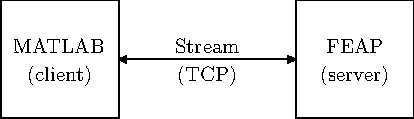
\includegraphics{commfig}
\end{center}

There are several advantages to this socket-based architecture:
\begin{itemize}
\item
  The text command interface to FEAP has remained more stable
  than the internal architecture.  By building the communication between
  MATLAB and FEAP on this text interface, rather than by calling FEAP's
  internal routines directly from MATLAB, it is less difficult to keep
  MATFEAP working with multiple FEAP versions than it was to keep FEAPMEX
  working.

\item
  When debugging problems with FEAP, it is possible to run {\tt gdb},
  {\tt valgrind}, and other debugging tools directly on the FEAP
  server.  Also, if FEAP crashes, it will not take MATLAB down with
  it.

\item
  Because each FEAP simulation runs in a separate process, there are no
  issues with initializing the global segment (and all the common
  block variables that FEAP uses) on initialization, nor are there
  issues with releasing system resources on exit.  In contrast,
  getting the global FEAP initialization and shutdown right was always
  tricky with FEAPMEX.

\item
  Also because each FEAP simulation runs in a separate process, it is
  possible to have multiple FEAP simulations open simultaneously.

\item
  The FEAP server does not need to be on the same machine as the MATLAB
  client.  This could be useful for running MATLAB on a laptop or other
  ``front-end'' machine and running the FEAP server on a higher-power
  remote system.

\item
  MATFEAP does not need a MEX component.  Therefore, there are no
  issues of compatibility with the compilers used by the MEX
  interface.  Users can compile the FEAP server using the same
  compilers and flags that they use to compile FEAP, and the client
  support code needs only MATLAB and Java.

\end{itemize}

\section{Code organization}

The server code is made up of three basic modules:
\begin{itemize}
\item 
  The server daemon module is responsible for setting up a socket
  connection on the server side, setting up a new child processes to handle
  each incoming simulation request, and cleaning up the child processes
  when simulations are finished.  The call to the server module is transparent
  from the perspective of the FORTRAN code that calls it.  When the server
  module returns control to a child process, that child communicates with
  the client via its standard input and output streams, just as it would
  if the client were someone entering commands at the terminal.

\item
  The {\tt feapsrv} module provides a command line interface for accessing
  FEAP's internal state, and implements the server side of the data transfer
  protocols used by MATFEAP.  This command line interface is invoked at
  the start of each simulation, and it can be invoked during the simulation
  through a FEAP user macro.

\item
  There are several FORTRAN support routines called by {\tt feapsrv}.
  Some of these routines are simple interfaces to ordinary FEAP
  functions; the rest are modifications to FEAP functions, mostly
  automatically generated.  These FORTRAN routines serve two purposes.
  First, they let us call a few FEAP routines from {\tt feapsrv}
  without worrying about proper cross-language binding of FEAP's
  common block variables.  Second, they add synchronization messages
  to existing routines in order to make it easy for the client to tell
  when input is expected.

\end{itemize}

In addition to the FORTRAN support routines, the server is also linked to
the standard FEAP library.

The support on the client side consists of two pieces: a Java class
that manages the socket connection (there is also an optional MEX
library), and a library of MATLAB routines that manage the protocol by
which MATLAB communicates with the FEAP server.

The documentation that follows is largely automatically extracted from
specially-formatted comments in the MATFEAP source files.  The documentation
tool we use is available at
\begin{verbatim}
  http://www.cims.nyu.edu/~dbindel/code/dsbweb.c
\end{verbatim}


\section{Running MATFEAP}

To run a MATFEAP simulation, you have to build the {\tt feaps} (FEAP
server) executable and run it on the machine where the simulation is
to take place.  Once the FEAP server is running, start MATLAB and
execute the {\tt matfeap\_init} script to set the system paths
correctly:
\begin{verbatim}
% matfeap_init.m
% Initializes paths used by the MATFEAP interface

addpath([pwd, '/mlab']);
cd mlab/csock
if exist('csockmex')
  fprintf('Using C socket bindings\n');
  cd ../..
  addpath([pwd, '/mlab/csock']);
  feaps_unix;
else
  fprintf('Using Java socket bindings\n');
  cd ../..
  addpath([pwd, '/mlab/jsock']);
  javaaddpath([pwd, '/mlab/jsock']);
  feaps_pipe;
end
\end{verbatim}


This initialization routine should work fine with MATLAB versions 7+,
including the student edition.  In MATLAB 6.5, the class path used by
MATLAB's JVM cannot be dynamically modified, so one has to set that
variable in another way -- see the Mathworks site for details.


\section{Simple example}

To give the flavor for how MATFEAP works in practice, we give a simple
example that uses several of MATFEAP's capabilities.

The {\tt Iblock2} input deck in the example subdirectory describes a
square mesh with {\tt n} elements on a side, where the parameter {\tt n}
is not defined in the input deck.  We start a FEAP simulation with
{\tt n = 10}, get the tangent stiffness and residual into MATLAB,
solve the linear system and write the results back to FEAP, and then
use FEAP's X11 graphics to show the displaced shape.  Once the user
has finished admiring our deformed block, he can press a key (at which
point the FEAP simulation will exit and the graphics will disappear).

\begin{verbatim}
param.n       = 10;  % Parameter to the FEAP input deck
param.verbose = 1;   % See everything that FEAP sends

p  = feapstart('Iblock2', param);  % Start FEAP simulation

K  = feaptang(p);    % Form the tangent matrix
R  = feapresid(p);   % Form the residual force vector
du = K\R;            % Compute a Newton update
feapsetu(p, du);     % Set the displacement vector

% Plot the results
feapcmd(p, 'plot', 'defo', 'mesh', 'boun', 'load', 'end');

% Quit
disp('Press any key to exit');
pause;
feapquit(p);

\end{verbatim}



% ===================================================================
\chapter{Setting up the C server}

The {\tt feapserver} routine provides a fairly generic way to turn a
console-based FORTRAN program into a UNIX server daemon.  From the
perspective of the FORTRAN program, very little changes on return from
a call to {\tt feapserver}, except that the input and output terminals
are now connected to a remote client via a socket.  Ordinary FORTRAN
{\tt read} and {\tt write} statements directed to the standard output
will go over that socket.  The caller doesn't need to know anything about
the details that turn the program into a network server daemon on this
call.  However, these details and their implementation are spelled out
below.

\section{Reaping child processes}

In UNIX, child processes are not released to the system until after the
parent process checks the child process exit status using {\tt wait} or
{\tt waitpid}.  We install a handler on SIGCHLD events (change of child
status) that checks the exit status of any child processes that are 
finished.

This is a standard piece of most UNIX daemons.

\begin{verbatim}
static void sigchld_handler(int s)
{
    while (waitpid(-1, NULL, WNOHANG) > 0);
}

static void install_reaper()
{
    struct sigaction sa;
    sa.sa_handler = sigchld_handler;
    sigemptyset(&sa.sa_mask);
    sa.sa_flags = SA_RESTART;
    ec(sigaction(SIGCHLD, &sa, NULL));
}

\end{verbatim}
\section{Receiving TCP socket connections}

On the server side, there are two phases to setting up a socket connection.
First, we need to set up a socket -- create it, give it an address with
{\tt bind}, and use {\tt listen} to tell the system that we can receive
connections on it.  By default, the server listens on {\tt MYPORT} (3490),
but this value can be changed by setting the {\tt MATFEAP\_PORT} environment
variable.

\begin{verbatim}
static int tcp_socket_setup(int port)
{
    int sockfd;                           /* socket file descriptor */
    struct sockaddr_in my_addr;           /* my address information */
    int yes=1;

    memset(&my_addr, 0, sizeof(my_addr));
    my_addr.sin_family = AF_INET;
    my_addr.sin_port = htons(port);
    my_addr.sin_addr.s_addr = INADDR_ANY;

    ec(sockfd = socket(AF_INET, SOCK_STREAM, 0));
    ec(setsockopt(sockfd, SOL_SOCKET, SO_REUSEADDR, &yes, sizeof(int)));
    ec(bind(sockfd, (struct sockaddr*) &my_addr, sizeof(my_addr)));
    ec(listen(sockfd, BACKLOG));

    printf("Server listening on port %d\n", port);
    return sockfd;
}

static int tcp_handle_connection(int sockfd)
{
    struct sockaddr_in their_addr;
    socklen_t sin_size = sizeof(struct sockaddr_in);
    while (1) {
        int new_fd = accept(sockfd, (struct sockaddr*) &their_addr, &sin_size);
        if (new_fd < 0)
            perror("accept");
        else {
            time_t c = time(NULL);
            printf("Connection from %s -- %s",
                   inet_ntoa(their_addr.sin_addr), ctime(&c));
            return new_fd;
        }
    }
}

\end{verbatim}
\section{Receiving local socket connections}

In addition to TCP socket connections, we allow the server to use
UNIX domain socket connections.  UNIX domain sockets are used in various
other system servers as well, including X11.  The primary advantage of
UNIX-domain sockets over TCP sockets is performance: if you're
going to run both the client and the server on the same machine and
you use a UNIX-domain socket, then the operating system can handle
context switches a little more intelligently.  The disadvantage of
using UNIX domain sockets is that Java doesn't know about them at
this time -- you have to use the MEX-based socket infrastructure to
connect to the UNIX domain server.

UNIX domain sockets differ from TCP sockets primarily in the setup
phase -- afterward, everything works the same.  The location of a
UNIX domain socket is specified as a filesystem location rather than
a port number.  We use the existence of a port name to tell MATFEAP
to listen on a UNIX domain socket.

\begin{verbatim}
static int local_socket_setup(const char* sockname)
{
    int sockfd;                           /* socket file descriptor */
    struct sockaddr_un my_addr;           /* my address information */
    int len;

    /* Remove any previous socket */
    unlink(sockname);

    memset(&my_addr, 0, sizeof(my_addr));
    my_addr.sun_family = AF_UNIX;
    strcpy(my_addr.sun_path, sockname);
    len = sizeof(my_addr.sun_family) + strlen(my_addr.sun_path) + 1;

    ec(sockfd = socket(AF_UNIX, SOCK_STREAM, 0));
    ec(bind(sockfd, (struct sockaddr*) &my_addr, len));
    ec(listen(sockfd, BACKLOG));

    printf("Server listening on local socket %s\n", sockname);
    return sockfd;
}

static int local_handle_connection(int sockfd)
{
    struct sockaddr_un their_addr;
    socklen_t sin_size = sizeof(struct sockaddr_un);
    while (1) {
        int new_fd = accept(sockfd, (struct sockaddr*) &their_addr, &sin_size);
        if (new_fd < 0)
            perror("accept");
        else {
            time_t c = time(NULL);
            printf("Connection -- %s", ctime(&c));
            return new_fd;
        }
    }
}

\end{verbatim}
\section{Deciding on a socket connections}

We decide whether to use TCP or UNIX domain sockets based on
the setting of the environment variables.  If
{\tt MATFEAP\_SOCKNAME} is set, we use that as the address for
a local UNIX-domain socket.  Otherwise, if {\tt MATFEAP\_PORT} is
set, we use that as the port number for a TCP-based socket.
If no relevant environment variable is set, then we default to
a TCP-based server listening on port 3490.

\begin{verbatim}
static int feapsock_local_socket;

static int socket_setup()
{
    int port = MYPORT;
    char* port_env = getenv(PORT_ENV_VAR);
    char* sockname = getenv(SOCKNAME_ENV_VAR);
    if (port_env)
        port = atoi(port_env);

    feapsock_local_socket = (sockname != 0);
    if (feapsock_local_socket)
        return local_socket_setup(sockname);
    else
        return tcp_socket_setup(port);
}

static int handle_connection(int sockfd)
{
    if (feapsock_local_socket)
        return local_handle_connection(sockfd);
    else
        return tcp_handle_connection(sockfd);
}

\end{verbatim}
\section{Redirecting I/O streams}

UNIX treats socket file descriptors like any other file
descriptors.  That means the socket input and output streams can be
connected to {\tt stdin} (fd 0) and {\tt stdout} (fd 1) using the
{\tt dup} or {\tt dup2} system calls.  I leave {\tt stderr} alone
so that the FEAP server can send debugging information to the terminal
without breaking the protocol used to communicate between the server and
the client.

\begin{verbatim}
static void send_std_to_socket(int new_fd)
{
    dup2(new_fd, 0);
    dup2(new_fd, 1);
    /*dup2(new_fd, 2);*/
    close(new_fd);
}

\end{verbatim}
\section{The main daemon}

The main loop is a Fortran-callable routine that accepts incoming
socket connections from clients and assigns to each a simulation
process.  The call to {\tt feapserver} in the original process
never exits.  In child processes created to handle incoming
connections, {\tt feapserver} returns control to the calling routine,
allowing FEAP to continue running as it usually would.

\begin{verbatim}
int feapserver_()
{
    int sockfd = socket_setup();
    install_reaper();

    while (1) {
        int new_fd = handle_connection(sockfd);
        if (!fork()) {  /* This is the child process */
            close(sockfd);
            send_std_to_socket(new_fd);
            return 0;
        }
        close(new_fd);  /* Parent doesn't need this */
    }

    exit(0);
}

\end{verbatim}



% ===================================================================
\chapter{The {\tt feapsrv} interface}

When running {\tt feapsrv}, the client can access most
MATFEAP-specific functions using a text-based command interface.
These include things like changing the working directory, setting FEAP
parameters, and sending or receiving FEAP's internal arrays and common
block entries.  The C code is in the driver's seat when {\tt feapsrv}
is active, though there are frequent calls back into the FORTRAN code.

\section{Synchronization}

In order to communicate over a socket, we need some protocol for telling
who is writing and who is reading.  Otherwise, it's easy to get into a
deadlock, where the client is trying to send a command while the server
is itself blocked on a send.  The {\tt feapsync} function sends a string
that can be used as a synchronization point by the client, so that (for
example) the client won't send one command until the previous command has
finished.  This isn't a perfect solution, but it is a useful primitive.

Synchronization messages are accompanied by an integer label -- 0 is
a sort of don't care label, and is what we use for all the synchronization
messages that aren't explicitly requested by the client.

The {\tt feapsync} routine is called in four places:
\begin{enumerate}
\item
During file name entry, the server sends a synchronization message
just before waiting on each read.  This is mostly so that I don't
have to recognize what constitutes a prompt for a filename
(the prompts changed between FEAP 7.x and 8.0).

\item
Just before requesting input during a {\tt tinput} call, the server
sends a synchronization message.  Like the previous class of messages,
these messages are mainly to prevent me from having to understand
what constitutes a prompt.

\item
The last message sent by the server before exit is a synchronization
message.  We use this to keep the client from closing the connection
too soon -- in a well-behaved shutdown, the client shouldn't close the
connection until that last message says that the server is ready.

\item
The client can explicitly request a labeled synchronization message
via the FEAP user macro {\tt serv}.
\end{enumerate}

\begin{verbatim}
int feapsync_(int* marker)
{
    printf("\nMATFEAP SYNC %d\n", *marker);
    fflush(stdout);
    return 0;
}

\end{verbatim}
\section{Type conversion}

Even on a single machine, we need to convert all binary data transfered
to wire format.  This is because the Java input functions assume wire
format independent of what architecture we use.  The {\tt hton[sl]} and
{\tt ntoh[ls]} functions convert between host and network long (32-bit)
and short (16-bit) integers, but there is no such standard function for
double precision floating point data.  This is what {\tt ntohd} and
{\tt htond} are for.

\begin{verbatim}
double ntohd(double x)
{
    double one = 1;
    if (*((char*) &one) == 0) {
        double tmp;
        char* src = (char*) &x;
        char* dst = (char*) &tmp;
        dst[0] = src[7];
        dst[1] = src[6];
        dst[2] = src[5];
        dst[3] = src[4];
        dst[4] = src[3];
        dst[5] = src[2];
        dst[6] = src[1];
        dst[7] = src[0];
        return tmp;
    } else {
        return x;
    }
}

double htond(double x)
{
    return ntohd(x);
}

\end{verbatim}
\section{Sending parameter values}

FEAP has a routine {\tt pconst()} that reads in parameter values, but it turns
out not to be optimal for MATFEAP for two reasons.  First, if the parameter
happens to be invalid, FEAP crashes -- not exactly the ideal behavior.
Second, {\tt pconst()} sends a prompt to the standard output, and that prompt
can screw up the message synchronization used by MATFEAP.

\begin{verbatim}
void feapsrv_param(const char* var, double val)
{
    extern int servparam_(int*, int*, double*);
    int i1;
    int i2;

    if (var[0] >= 'A' && var[0] <= 'Z')
       i1 = 1+var[0]-'A';
    else if (var[0] >= 'a' && var[0] <= 'z')
       i1 = 1+var[0]-'a';
    else
       return;  /* Invalid name */

    if (var[1] == '\0')
        i2 = 0;
    else if (var[1] >= 'A' && var[1] <= 'Z')
        i2 = 1+(var[1]-'A');
    else if (var[1] >= 'a' && var[1] <= 'z')
        i2 = 1+(var[1]-'a');
    else if (var[1] >= '0' && var[1] <= '9')
        i2 = 27+(var[1]-'0');
    else
        return;  /* Invalid name */

    servparam_(&i1, &i2, &val);
}


\end{verbatim}
\section{Sending binary arrays}

To send an array to the client, we use the following protocol.
\begin{enumerate}
\item Server sends: {\tt Send {\it type} {\it count}}, where
{\it type} is {\tt i} (integer) or {\tt d} (double), and
{\it count} is an integer indicating the number of values to
be sent.
\item Client sends: {\tt text} or {\tt binary} or {\tt cancel}.
\item Server sends: nothing if the client requested {\tt cancel}; a
stream of 32-bit integers or 64-bit doubles in wire format if the
client requested {\tt binary}; or ordinary text representations of
the array data, printed one per line, if the client requested
{\tt text}.
\end{enumerate}

All this assumes that the array was found -- if not, the server would
send {\tt Not found} instead of sending a {\tt Send} line, and the
interaction would stop there.

\begin{verbatim}
int fmsendint_(int* data, int* len)
{
    char buf[256];
    char* token;
    int i;

    printf("Send int %d\n", *len);
    fflush(stdout);
    if (fgets(buf, sizeof(buf), stdin) == NULL)
        return 0;

    token = strtok(buf, " \t\r\n");
    if (strcmp(token, "text") == 0) {
        for (i = 0; i < *len; ++i)
            printf("%d\n", data[i]);
    } else if (strcmp(token, "binary") == 0) {
        for (i = 0; i < *len; ++i) {
            int32_t datum = htonl(data[i]);
            fwrite(&datum, sizeof(int32_t), 1, stdout);
        }
    }
    fflush(stdout);

    return 0;
}

int fmsenddbl_(double* data, int* len)
{
    char buf[256];
    char* token;
    int i;

    printf("Send double %d\n", *len);
    fflush(stdout);
    if (fgets(buf, sizeof(buf), stdin) == NULL)
        return 0;

    token = strtok(buf, " \t\r\n");
    if (strcmp(token, "text") == 0) {
        for (i = 0; i < *len; ++i)
            printf("%g\n", data[i]);
    } else if (strcmp(token, "binary") == 0) {
        for (i = 0; i < *len; ++i) {
            double datum = htond(data[i]);
            fwrite(&datum, sizeof(double), 1, stdout);
        }
    }
    fflush(stdout);

    return 0;
}

\end{verbatim}
\section{Receiving binary arrays}

To receive an array to the client, we use a protocol very similar
to the one used for sending:
\begin{enumerate}
\item Server sends: {\tt Recv {\it type} {\it count}}, where
{\it type} is {\tt i} (integer) or {\tt d} (double), and
{\it count} is an integer indicating the number of values to
be sent.
\item Client sends: {\tt text} or {\tt binary} or {\tt cancel}.
\item Client sends: nothing if the client requested {\tt cancel}; a
stream of 32-bit integers or 64-bit doubles in wire format if the
client requested {\tt binary}; or ordinary text representations of
the array data, printed one per line, if the client requested
{\tt text}.
\end{enumerate}

All this assumes that the array was found -- if not, the server would
send {\tt Not found} instead of sending a {\tt Send} line, and the
interaction would stop there.

It is much more likely that a receive request will be canceled than
that a send request will be canceled.  When the client wants to receive
some data, it dynamically allocates as much space as needed to hold
the response; but when the client wants to send data, it has to send
exactly as much as the FEAP array wants.

\begin{verbatim}
int fmrecvint_(int* data, int* len)
{
    char buf[256];
    char* token;
    int i;

    printf("Recv int %d\n", *len);
    fflush(stdout);
    if (fgets(buf, sizeof(buf), stdin) == NULL)
        return 0;

    token = strtok(buf, " \t\r\n");
    if (strcmp(token, "text") == 0) {
        for (i = 0; i < *len; ++i)
            scanf("%d", &(data[i]));
    } else if (strcmp(token, "binary") == 0) {
        for (i = 0; i < *len; ++i) {
            int32_t datum;
            fread(&datum, sizeof(int32_t), 1, stdin);
            data[i] = ntohl(datum);
        }
    }

    return 0;
}

int fmrecvdbl_(double* data, int* len)
{
    char buf[256];
    char* token;
    int i;

    printf("Recv double %d\n", *len);
    fflush(stdout);
    if (fgets(buf, sizeof(buf), stdin) == NULL)
        return 0;

    token = strtok(buf, " \t\r\n");
    if (strcmp(token, "text") == 0) {
        for (i = 0; i < *len; ++i)
            scanf("%lg", &(data[i]));
    } else if (strcmp(token, "binary") == 0) {
        for (i = 0; i < *len; ++i) {
            double datum;
            fread(&datum, sizeof(double), 1, stdin);
            data[i] = ntohd(datum);
        }
    }

    return 0;
}

\end{verbatim}
\section{Sending sparse arrays}

Sparse arrays are sent from FEAP to MATLAB in coordinate form.  Transfer
from MATLAB back to FEAP is currently not supported.  There was already
a FORTRAN routine in place to print various FEAP sparse matrices to a
file for later retrieval in MATLAB; I adapted that routine for use in
MATFEAP by changing all the file I/O routines into calls to {\tt writeaij}
(below).  Sending an array consists of two steps: 
\begin{enumerate}
\item 
A call to {\tt matspew} to accumulate a count of the number
of nonzero coordinates to be sent during the data transfer.
After making the count, we send a message {\tt nnz {\it count}} to
the client.
\item 
A second call to {\tt matspew} to send the data.  For the binary version
of the protocol, the data is sent in triplets: {\tt i, j, Aij},
where {\tt i} and {\tt j} are 32-bit integers in wire format and
{\tt Aij} is a wire format double.  For text versions of the protocol,
the data is sent with one triple per line.
\end{enumerate}

\begin{verbatim}
int writeaij_(int* i, int* j, double* aij, int* count)
{
    /* Cases:
     *  count >=  0 -- accumulate count
     *  count == -1 -- output as text
     *  count == -2 -- output as binary
     */
    if (*count >= 0) {
        ++(*count);
    } else if (*count == -1) {
        printf("%d %d %lg\n", *i, *j, *aij);
    } else if (*count == -2) {
        double coord[3];
        coord[0] = htond(*i);
        coord[1] = htond(*j);
        coord[2] = htond(*aij);
        fwrite(coord, sizeof(double), 3, stdout);
    }
    return 0;
}

void sparse_write(char* types, char* var)
{
    extern int matspew_(char* var, int* cnt);
    int type = 0;
    if (strcmp(types, "text") == 0)
        type = -1;
    else if (strcmp(types, "binary") == 0)
        type = -2;
    if (type && var) {
        int cnt = 0;
        matspew_(var, &cnt);
        printf("nnz %d\n", cnt);
        cnt = type;
        matspew_(var, &cnt);
    }
}

\end{verbatim}
\section{The {\tt feapsrv} dispatcher}

The {\tt feapsrv} routine is called both at the beginning of the
MATFEAP run and whenever the user macro {\tt serv} is invoked.
This routine provides a common interface for receiving and dispatching
most of the commands used by MATFEAP.  In order to keep me honest --
and in order to aid debugging -- I have tried to make it possible to
use the {\tt feapsrv} subcommands as an ordinary user at a terminal
interface.  This means, among other things, that there is a help string.

\begin{verbatim}
char* FEAPSRV_HELP = 
    "Commands are:\n"
    "  start           - Start / resume ordinary FEAP interaction\n"
    "  quit            - Terminate this FEAP process\n"
    "  help            - Get this message\n"
    "  cd DIR          - Change to directory DIR\n"
    "  cd              - Print current working directory\n"
    "  param           - Set FEAP parameters\n"
    "  set VAR         - Set FEAP common block variable\n"
    "  get VAR         - Print FEAP common block variable\n"
    "  getm VAR        - Start get of FEAP array\n"
    "  setm VAR        - Start set FEAP array\n"
    "  sparse FMT VAR  - Get FEAP sparse matrix as binary or text\n"
    "  clear_isformed  - Clear with the 'resid formed' flag\n"
    "\n"
    "You can enter server mode from FEAP using the 'serv' macro.\n"
    "See the source code / documentation for more information on the\n"
    "protocols used to exchange arrays and sparse matrices\n";

int feapsrv_()
{
    char buf[256];
    printf("FEAPSRV>\n");
    fflush(stdout);
    while (fgets(buf, sizeof(buf), stdin) != NULL) {
        char* token = strtok(buf, " \t\r\n");
        if (token == NULL) {
            continue;
        } else if (strcmp(token, "start") == 0) {
            return 0;
        } else if (strcmp(token, "quit") == 0) {
            exit(0);
        } else if (strcmp(token, "help") == 0) {
            printf(FEAPSRV_HELP);
        } else if (strcmp(token, "cd") == 0) {
            token = strtok(NULL, " \t\r\n");
            if (token == NULL) 
                printf("PWD: %s\n", getcwd(buf, sizeof(buf)));
            else if (chdir(token) < 0)
                perror("chdir");
        } else if (strcmp(token, "param") == 0) {
            char* name = strtok(NULL, " \t\r\n");
            char* valtok = strtok(NULL, " \t\r\n");
            double val = atof(valtok);
            feapsrv_param(name, val);
        } else if (strcmp(token, "set") == 0) {
            extern int feapget_(char* var, char* mode);
            token = strtok(NULL, " \t\r\n");
            if (token) {
                int n = strlen(token);
                token[n] = ' ';
                feapget_(token, "w");
                token[n] = 0;
            }
        } else if (strcmp(token, "get") == 0) {
            extern int feapget_(char* var, char* mode);
            token = strtok(NULL, " \t\r\n");
            if (token) {
                int n = strlen(token);
                token[n] = ' ';
                feapget_(token, "r");
                token[n] = 0;
            }
        } else if (strcmp(token, "getm") == 0) {
            extern int feapgetm_(char* var, int len);
            token = strtok(NULL, " \t\r\n");
            if (token)
                feapgetm_(token, strlen(token));
        } else if (strcmp(token, "setm") == 0) {
            extern int feapsetm_(char* var, int len);
            token = strtok(NULL, " \t\r\n");
            if (token)
                feapsetm_(token, strlen(token));
        } else if (strcmp(token, "sparse") == 0) {
            char* transfertype = strtok(NULL, " \t\r\n");
            char* varname = strtok(NULL, " \t\r\n");
            if (transfertype && varname)
                sparse_write(transfertype, varname);
        } else if (strcmp(token, "clear_isformed") == 0) {
            extern int feaptformed_();
            feaptformed_();
        } else {
            printf("Unrecognized command: %s\n", token);
        }
        printf("FEAPSRV>\n");
        fflush(stdout);
    }
    return 0;
}
\end{verbatim}



% ===================================================================
\chapter{FORTRAN support routines}

The FORTRAN support routines really play a secondary role to the C routines.
They are almost all either modifications of existing FEAP routines or thin
wrappers over top of existing FEAP routines.  The main reason that some of
these routines exist is that it is {\em much} easier to access the FORTRAN
common block data used by FEAP directly from FORTRAN than it is to access 
it from C.

\section{Adding synchronization on input}

We have our own version of the input routine {\tt tinput},
which mediates most of the console input in FEAP.  Our version
calls {\tt feapsync} to allow the client to sync up with the
server, then calls {\tt tinput2}, which is generated from the
ordinary {\tt tinput} routine in FEAP.

\begin{verbatim}
      logical function tinput(tx,mt,d,nn)

      include  'iofile.h'

      logical   tinput2
      integer   mt,nn,bnum
      character tx(*)*15
      real*8    d(*)

      save

      if(ior.lt.0) then
        bnum = 0
        call feapsync(bnum)
      end if
      tinput = tinput2(tx,mt,d,nn)

      end
\end{verbatim}
\section{Getting and setting scalars}

The {\tt feapget} routine either reads a common block variable from
the standard input or writes a common block variable to the 
standard output, depending on whether the mode is {\tt r} or {\tt w}.
If no such variable is available, the routine doesn't do anything.
The data is always sent in text format.

NOTE:  The FORTRAN {\tt read} statement is not very smart, so if
the client tries to write a double value into an integer variable,
the FORTRAN I/O library is likely to complain and abort the program.

\begin{verbatim}
      subroutine feapget(var, mode)
\end{verbatim}
\section{Sending matrices}

The {\tt feapgetm(var)} command fetches the named array from
FEAP's dynamic memory system using {\tt pgetd}.   If the array
is found, {\tt feapgetm} calls {\tt feapsendint} or {\tt feapsenddbl}
in order to return the data to the client.  Otherwise, it prints
a ``Not found'' message.

There are two variants of this routine.  The code below works with
newer versions of FEAP (8.0+) in which the {\tt p\_point.h} header
declares an integer variable capable of storing a FEAP pointer.
The code in {\tt feapgetm7.f} works with earlier versions of FEAP
in which pointers are always represented as 32-bit integers.

\begin{verbatim}
      subroutine feapgetm(var)

      implicit  none

      include 'comblk.h'
      include 'pointer.h'
      include 'p_point.h'

      character var*(*)
      logical flag
      integer lengt, prec

      save

      call pgetd( var, point, lengt, prec, flag )
      if(flag) then
        if(prec.eq.1) then
          call fmsendint(mr(point), lengt)
        else
          call fmsenddbl(hr(point), lengt)
        endif
      else
        print *, 'Not found'
      endif

      end
\end{verbatim}
\section{Receiving matrices}

The {\tt feapsetm} command is exactly analogous to {\tt feapgetm},
except that it receives data from the client using {\tt feaprecvint}
and {\tt feaprecvdbl} where {\tt feapgetm} sends data. 

\begin{verbatim}
      subroutine feapsetm(var)
\end{verbatim}
\section{FORTRAN sparse matrix output support}

The {\tt matspew} command is based on the sparse matrix output
routine available at {\tt www.ce.berkeley.edu/\~{}rlt/feap/umacr3.f}.
The {\tt matspew} routine differs from the original routine
primarily in that it calls a function {\tt writeaij} where the
original routine would write a coordinate triple to file.
The {\tt writeaij} routine takes {\tt i}, {\tt j}, and {\tt Aij},
but it also takes an additional argument that controls the precise
behavior of the routine -- if negative, it tells {\tt writeaij}
to write binary or text data.  If the argument is non-negative,
{\tt writeaij} writes no output, but increments the argument with
each call in order to compute the number of nonzeroes that would
be written.

The routine can output the following matrices:
\begin{itemize}
\item Tangent ({\tt tang}) and unsymmetric tangent( {\tt utan})
\item Consistent mass ({\tt mass} or {\tt cmas}), lumped mass
({\tt lmas}), or unsymmetric mass ({\tt umas})
\item Consistent damping ({\tt damp} or {\tt cdam})
or unsymmetric damping ({\tt udam})
\end{itemize}

\begin{verbatim}
      subroutine matspew(lct, cnt)
\end{verbatim}
\section{Clearing the solution flag}

The FEAP common block flag {\tt fl(8)} is used to keep track of
whether or not the residual has been formed since the last {\tt solv}
call.  If it has already been formed, there's no reason to form it
again.  But when we do a calculation on MATLAB and directly write
to the FEAP vectors containing the current state, whatever residual
might be in FEAP's memory is invalidated.  We therefore use 
{\tt feaptformed} to clear the value of {\tt fl(8)} so that FEAP
will know when such an event has happened.

\begin{verbatim}
      subroutine feaptformed()

      implicit  none

      include  'fdata.h'

      save

      fl(8) = .false.

      end
\end{verbatim}
\section{The FEAP dispatch macro}

The FEAP user macro {\tt serv} plays two roles.  If called with
a positive integer argument (e.g. {\tt serv,,1}), FEAP will call
{\tt feapsync} to output a string that the MATLAB client can
use for synchronization.  Otherwise, FEAP will call the {\tt feapsrv}
dispatcher routine, which allows the MATLAB client to access most of
the MATFEAP-specific functionality available.

\begin{verbatim}
      subroutine umacr1(lct,ctl,prt)

c      * * F E A P * * A Finite Element Analysis Program

c....  Copyright (c) 1984-2006: Regents of the University of California
c                               All rights reserved

c-----[--.----+----.----+----.-----------------------------------------]
c     Modification log                                Date (dd/mm/year)
c       Original version                                    01/11/2006
c-----[--.----+----.----+----.-----------------------------------------]
c      Purpose:  User interface for adding solution command language
c                instructions.

c      Inputs:
c         lct       - Command character parameters
c         ctl(3)    - Command numerical parameters
c         prt       - Flag, output if true

c      Outputs:
c         N.B.  Users are responsible for command actions.  See
c               programmers manual for example.
c-----[--.----+----.----+----.-----------------------------------------]
      implicit  none

      include  'iofile.h'
      include  'umac1.h'

      logical   pcomp,prt
      character lct*15
      real*8    ctl(3)
      integer   ival

      save

c     Set command word

      if(pcomp(uct,'mac1',4)) then      ! Usual    form
        uct = 'serv'                    ! Specify 'name'
      elseif(urest.eq.1) then           ! Read  restart data

      elseif(urest.eq.2) then           ! Write restart data

      else                              ! Perform user operation
        ival = ctl(1)
        if(ival.gt.0) then
          call feapsync(ival)
        else
          call feapsrv()
        endif
      endif

      end
\end{verbatim}
 \section{Generated files}

 We mostly augment FEAP by adding new files, but there are a few minor
 changes that we have to make to the existing files as well.  Because
 MATFEAP is supposed to work with different versions of FEAP, and because
 some of the files we need to modify vary between FEAP versions, we
 automatically rewrite the FEAP sources with scripts, rather than trying
 to come up with a one or more modified routine that will be compatible with
 all the relevant versions.

 The most obvious change is to the FEAP front-end routine.  We add calls
 to {\tt feapserver} (to start the socket server) and to {\tt feapsrv}
 (so that the user can set parameters, change directories, etc. before
 entering filenames and processing the input file.

\begin{verbatim}

feap.f: $(FEAPMAIN)
        $(AWK) ' \
        /call pstart/ { \
          print "      call feapserver()"; \
          print "      call feapsrv()" } \
        { print }' $(FEAPMAIN) > feap.f

\end{verbatim}
 FEAP calls the {\tt plstop} routine to close files, clear memory, and
 otherwise clean up before exiting.  It causes problems on some systems
 to close the socket connection before FEAP finishes writing whatever
 it will to the standard output, so we add a synchronization call at
 the very end of {\tt plstop}, just before the true exit.

\begin{verbatim}
plstop.f: $(PLSTOP)
        $(AWK) ' \
        /^[ ]*stop/ { print "      call feapsync(1)" } \
        { print }' $(PLSTOP) > plstop.f

\end{verbatim}
 The {\tt filnam} routine, which reads in file names from the standard
 input, requires four modifications:
 \begin{enumerate}
 \item  We need to make sure that
   {\tt filnam} doesn't decide to use the default file names saved in the
   {\tt feapname} file (which is what the ordinary FEAP routine does).
   So we strategically insert the statement {\tt lfil = .false.} (indicating
   that there's no {\tt feapname} to read) immediately before where FEAP
   tests {\tt lfil}.  
 \item   We add initialization routines for the
   various filename variables, fixing a bug in FEAP that would otherwise
   cause the program to go into a tailspin if we tried to quit rather than
   entering filenames.  
 \item  We make a call to {\tt cleannam} to turn any
   carriage returns and line feeds received by FEAP into ordinary spaces
   (it's unclear to me why these characters show up when I send the data
   over a socket and not over the terminal, but it seems that they do).
 \item   We add a call to {\tt feapsync} before each
   read, so that the client will know when it's supposed to provide input.
 \end{enumerate}

\begin{verbatim}
filnam.f:
        $(AWK) ' \
        /if\(lfil\) then/          { print "      lfil = .false."; init = 1 } \
        init == 1 && /^      else/ { init = 2 } \
        init == 2 && /^[ ]*p/      { print; sub(/ p/, " f") } \
        init == 2 && /^[ ]*end/    { init = 0 } \
        /^[0-9 \t]*read/           { print "      call feapsync(0)" } \
        /.not.pcomp\(filein/       { print "      call cleannam(filein)" }  \
        { print }' $(FEAPHOME)/program/filnam.f > filnam.f

\end{verbatim}
 The {\tt tinput} routine mediates most (though not all) of 
 FEAP's standard input.  Prior to version 8.0, {\tt tinput} was in the
 program subdirectory.  Since 8.0, there has been a special UNIX version
 of {\tt tinput} that uses a {\tt select} loop to keep X11 plots up to
 date while waiting for user input at the console.  We just need to
 find the version that's appropriate, copy it to the local directory,
 and rename it to {\tt tinput2}.  We have our own version of {\tt tinput}
 that will call {\tt tinput2} and then call {\tt feapsync} to allow
 the client to synchronize with the server.
\begin{verbatim}
tinput2.f: 
        if grep "function tinput" $(FEAPHOME)/program/*.f > /dev/null ; \
                then cp $(FEAPHOME)/program/tinput.f tinput0.f ; \
                else cp $(FEAPHOME)/unix/tinput.f tinput0.f ; \
                fi
        $(AWK) '{ gsub(/tinput/, "tinput2"); print }' tinput0.f > tinput2.f
        rm tinput0.f

\end{verbatim}



% ===================================================================
\chapter{MATLAB client}

The MATLAB client uses a thin Java client class to manage sending and
receiving data over a pipe or TCP socket.  There is also a C-language
MEX file which can be compiled to send and receive data over a TCP or
UNIX-domain socket (this C language MEX file is required to run
MATFEAP with Octave).  Except when using the {\tt feapsrv} interface,
the protocol is that the FEAP server will send a synchronization
method whenever it is waiting for input and when it is ready to quit.
In this mode, the client does not send data except immediately after
receiving a synchronization message from FEAP.

When using the {\tt feapsrv} interface documented previously, the generic
protocol is to wait for the {\tt FEAPSRV} prompt, then send a command, then
wait for the next {\tt FEAPSRV} prompt.  However, there are more elaborate
protocols for transferring arrays between FEAP and MATLAB, and these are
documented along with the {\tt feapsrv} module.

\section{Communication performance}

Of the three communication models offered by MATFEAP, the TCP socket
communication is the most flexible (since it can connect to servers on
remote machines).  At the same time, for single-machine use, it is the
slowest of the methods.  On the UNIX and OS X boxes where I have done
tests, both the pipe communication mechanism and the UNIX-domain
socket mechanism seem to achieve reasonable performance.  The default
behavior as set in {\tt matfeap\_init} is to use UNIX-domain sockets
with the C MEX client, and pipes with the Java client.

\section{Interface to the Java socket helper}

The Java socket helper class is a thin layer that lets us use
Java stream descriptors and binary I/O routines.  We use it to
establish socket connections, send an recieve lines of data,
etc.

The socket routines are
\begin{itemize}
\item {\tt sock\_new(hostname,port)} - start a socket connection
\item {\tt sock\_new(command)} - start a pipe connection
\item {\tt sock\_close(js)} - close a socket
\item {\tt sock\_recv(js)} - read a line of data
\item {\tt sock\_send(js)} - send a line of data
\item {\tt sock\_readdarray(js, len)} - read {\tt len} 64-bit doubles
into an array
\item {\tt sock\_readiarray(js, len)} - read {\tt len} 32-bit integers
into an array
\item {\tt sock\_senddarray(js, array)} - send an array of 64-bit doubles
\item {\tt sock\_sendiarray(js, array)} - send an array of 32-bit integers
\end{itemize}

\section{Interface to the C socket helper}

The C socket library provides a MEX interface to both TCP and
UNIX domain sockets.  This library can be used with MATLAB as an
alternative to the Java socket library; or it can be used with
recent versions of Octave. 

The C socket routines are identical to the Java socket routines,
save for {\tt sock\_new}:
\begin{itemize}
\item {\tt sock\_new(hostname,port)} - start a TCP socket connection
\item {\tt sock\_new(sockname)} - start a UNIX socket connection
\end{itemize}

In addition, we provide a routine that queries the environment to
figure out an appropriate name for a UNIX-domain socket to the server:
\begin{itemize}
\item {\tt sock\_default\_unix} - return the default UNIX socket name
\end{itemize}
\section {Communication setup}

These routines are used to specify which of the three communication modes
available to MATFEAP should be used.

\subsection{Setting up pipe communication}

The {\tt feaps\_pipe} function tells MATFEAP to manage communication
over a bidirectional pipe managed by Java.  This method is not
available in the C interface -- there the prefered connection method is
a UNIX-domain socket.

The default location for the FEAP executable used by in pipe mode is
{\tt {\it MATFEAP}/srv/feapp}.  The location of the {\tt feaps\_pipe.m}
file should be {\tt {\it MATFEAP}/srv/feaps\_pipe.m}.  Since the latter
file is obviously on the MATLAB path, we can get the fully qualified
name from MATLAB and extract the location of the MATFEAP home directory
from it.

\begin{verbatim}
function feaps_pipe(cmd)

global matfeap_globals
matfeap_globals.sockname = [];
matfeap_globals.server   = [];
matfeap_globals.port     = [];

if nargin < 1
  s = which('feaps_pipe.m');
  i = strfind(s, 'feaps_pipe.m')-length('mlab/');
  matfeap_globals.command = [s(1:i-1), 'srv/feapp'];
  fprintf('Using FEAP in pipe mode: %s\n', matfeap_globals.command);
elseif isempty(cmd)
  matfeap_globals.command = [];
  fprintf('Turning off FEAP pipe mode\n');
else
  matfeap_globals.command = cmd;
end

\end{verbatim}
\subsection{Setting up TCP socket communication}

The {\tt feaps\_tcp} function tells MATFEAP to manage communication
over a TCP socket (which may be managed by Java or C).  The default
location for the server is the local host on port 3490.

\begin{verbatim}
function feaps_tcp(server, port)

global matfeap_globals
matfeap_globals.command  = [];
matfeap_globals.sockname = [];
matfeap_globals.server   = [];
matfeap_globals.port     = [];

if nargin < 1
  matfeap_globals.server = '127.0.0.1';
  matfeap_globals.port   = 3490;
elseif nargin == 1
  if isempty(server)
    fprintf('Turning off FEAP TCP mode\n');
    return;
  elseif isnumeric(server)
    matfeap_globals.server = '127.0.0.1';
    matfeap_globals.port   = server;
  else
    matfeap_globals.server = server;
    matfeap_globals.port   = 3490;
  end
else
  matfeap_globals.server = server;
  matfeap_globals.port   = port;
end

fprintf('Using FEAP in TCP mode: %s:%d\n', ...
        matfeap_globals.server, matfeap_globals.port);

\end{verbatim}
\subsection{Setting up UNIX socket communication}

The {\tt feaps\_unix} function tells MATFEAP to manage communication
over a UNIX-domain socket.  This option is only available with the C
interface.  UNIX-domain sockets are identified by filesystem locations,
typically placed under {\tt /tmp}.  For MATFEAP, we use the default
name {\tt /tmp/feaps-{\it USER}}, where {\it USER} is the user name in
the current environment.  Because MATLAB doesn't have direct access to
the environment, we fetch the default socket name through the wrapper
function {\tt sock\_default\_unix}.

\begin{verbatim}
function feaps_unix(sockname)

global matfeap_globals
matfeap_globals.command  = [];
matfeap_globals.sockname = [];
matfeap_globals.server   = [];
matfeap_globals.port     = [];

if nargin < 1
  matfeap_globals.sockname = sock_default_unix;
elseif nargin == 1
  if isempty(sockname)
    fprintf('Turning off FEAP UNIX mode\n');
    return;
  else
    matfeap_globals.sockname = sockname;
  end
end

fprintf('Using FEAP on UNIX socket: %s\n', matfeap_globals.sockname);

\end{verbatim}
\section{Starting FEAP}

The {\tt feapstart} command is used to launch a new FEAP process:
\begin{verbatim}
function p = feapstart(fname, params)
\end{verbatim}

The file name argument is required.  The optional {\tt params}
argument plays double duty: a set of special parameters are used
to control things about the MATFEAP interface, and the remaining
parameters are used to initialize the FEAP variable list before
opening the designated input deck.
\subsection{Merging global parameters}

The {\tt matfeap\_globals} variable is used to provide default
values for the fields in the {\tt params} structure, if explicit
values are not otherwise provided.

\begin{verbatim}
global matfeap_globals;

if isstruct(matfeap_globals)
  if isempty(params)
    params = matfeap_globals;
  else
    pnames = fieldnames(matfeap_globals);
    for k = 1:length(pnames)
      if ~isfield(params, pnames{k})
        pvalue = getfield(matfeap_globals, pnames{k});
        params = setfield(params, pnames{k}, pvalue);
      end
    end
  end
end

\end{verbatim}
\subsection{Special parameters}

The special parameters are
\begin{itemize}
\item {\tt verbose}: if true, output all the stuff that FEAP sends
\item {\tt server} and {\tt port}: the server host name
(string) and port number (integer)
\item {\tt command}: if defined, this string says how to
execute the extended FEAP directly from the command line.
Used as an alternative to opening a socket connection.
\item {\tt dir}: the starting directory to change to after
connecting to the FEAP server.  By default we use the
client's present working directory.
\end{itemize}

At the same time we process these parameters, we remove them
from the {\tt param} structure.  That way, everything remaining
in the {\tt param} structure after this step can be interpreted
as a FEAP input parameter.

\begin{verbatim}
verb    = 0;           % Are we in verbose mode?
server  = '127.0.0.1'; % Server where FEAP is located
port    = 3490;        % Port where FEAP is located
dir     = pwd;         % Base directory to use for rel paths
command = [];          % Command string to use with pipe interface
sockname = [];         % UNIX domain socket name

if ~isempty(params)
  if isfield(params, 'verbose')
    verb = params.verbose;
    params = rmfield(params, 'verbose');
  end
  if isfield(params, 'server')
    server = params.server;
    params = rmfield(params, 'server');
  end
  if isfield(params, 'port')
    port = params.port;
    params = rmfield(params, 'port');
  end
  if isfield(params, 'command')
    command = params.command;
    params = rmfield(params, 'command');
  end
  if isfield(params, 'sockname')
    sockname = params.sockname;
    params = rmfield(params, 'sockname');
  end
  if isfield(params, 'dir')
    dir = params.dir;
    params = rmfield(params, 'dir');
  end
end


\end{verbatim}
\subsection{Input deck directory}

I assume that the file name does not contain any slashes or
backslashes; if those occur in the input deck name, then we'll
split the name argument into {\tt pathname} and {\tt fname}.

\begin{verbatim}
lastslash = max([strfind(fname, '/'), strfind(fname, '\')]);
if ~isempty(lastslash)
  pathname = fname(1:lastslash-1);
  fname = fname(lastslash+1:end);
else
  pathname = [];
end


\end{verbatim}
\subsection{Opening FEAP}

If {\tt sockname} is nonempty, then the user has specified
a UNIX domain socket to connect to the FEAP server.  Otherwise
if {\tt command} is nonempty, then the user has specified the
name of a command to start the (extended) FEAP.  This FEAP
executable has the same interface as the socket-based version,
but it communicates using the ordinary standard I/O streams,
which we will connect to a pipe.  Otherwise, we'll try to
communicate with the server via TCP.  We give the same generic error
message in the event of any error -- ``is the server there?''

Once a connection to the FEAP process has been established,
we save the relevant Java helper (or C handle) and the verbosity flag 
together in a handle structure.  This structure is the first argument 
to all the high-level MATFEAP interface functions.

\begin{verbatim}
try
  if ~isempty(sockname)
    fd = sock_new(sockname);
  elseif ~isempty(command)
    fd = sock_new(command);
  else
    fd = sock_new(server, port);
  end
catch
  fprintf('Could not open connection -- is the FEAP server running?\n');
  error(lasterr);
end

p = [];
p.fd = fd;
p.verb = verb;

\end{verbatim}
\subsection{Passing parameters}

The {\tt param} command in the {\tt feapsrv} interface allows the
user to send parameters to FEAP.  Parameter assignments have the
form ``param var val''.  Invalid assignments are (perhaps suboptimally)
simply ignored.

\begin{verbatim}
feapsrvp(p);
if ~isempty(params)
  pnames = fieldnames(params);
  for k = 1:length(pnames)
    pvar = pnames{k};
    pval = getfield(params, pnames{k});
    if ~isnumeric(pval)
      fprintf('Ignoring non-numeric parameter %s\n', pvar);
    else
      sock_send(fd, sprintf('param %s %g', pvar, pval));
      feapsrvp(p);
    end
  end
end

\end{verbatim}
\subsection{Setting the current directory}

If a home directory was specified via a {\tt dir} special
argument, we first change to that directory (by default, we
change to the client's present working directory).  If a path was
specified as part of the input deck name, we then change to that
directory.  If both {\tt dir} and {\tt pathname} are non-empty
and the {\tt pathname} specifies a relative path, we will end up
in the path relative to the specified base directory.

The {\tt feapsrv} command to change directories will return a
diagnostic message if for any reason the directory change doesn't
go through.  We ignore said message.

\begin{verbatim}
if ~isempty(dir)
  sock_send(fd, ['cd ', dir]);
  feapsrvp(p);
end
if ~isempty(pathname)
  sock_send(fd, ['cd ', pathname]);
  feapsrvp(p);
end

\end{verbatim}
\subsection{Sending the file names}

Once we've set up the parameter string and changed to the proper
directory, we're ready to actually start processing an input
deck.  The {\tt start} command gets us out of the {\tt feapsrv}
interface and into ordinary FEAP interactions.  We now need to
send to FEAP:
\begin{enumerate}
\item
The name of the input deck.
\item
Blank lines to say ``we accept the default names for the
auxiliary files.''  The number of auxiliary files has changed
over time, which is why we don't use a counter -- we just send
a blank line at every synchronization message until we see a
string that indicates that we've entered all the desired file
names.
\item
A string ``y'' for when we're asked if the file names are
correct.
\end{enumerate}

If an error occurs during entering the file name, we send the
``quit'' string and get out of dodge.  In response to a request
to quit, FEAP will go through the ordinary shutdown procedure,
so we'll wait for the last synchronization message before closing
the connection.

\begin{verbatim}
sock_send(fd, 'start');
feapsync(p);
sock_send(fd, fname);

doneflag = 0;
while 1
  s = sock_recv(fd);
  if strfind(s, '*ERROR*')
    p.verb = 1;
    feapsync(p);
    sock_send(fd, 'quit');
    feapsync(p);
    sock_close(fd);
    p = [];
    return;
  elseif strfind(s, 'Files are set')
    feapdispv(p, s);
    feapsync(p);
    sock_send(fd, 'y')
    feapsync(p);
    return;
  elseif strfind(s, 'MATFEAP SYNC')
    sock_send(fd, '');
  else
    feapdispv(p, s);
  end
end
\end{verbatim}
\section {User commands}

These are the main routines in the interface used directly by MATFEAP
users.

\subsection{Invoking FEAP macro commands}

The {\tt feapcmd} routine is used to invoke FEAP macro routines.
It's up to the user to ensure that after the end of the last command
in the list, FEAP is back at a prompt involving a {\tt tinput}
command (e.g. the macro prompt or a plot prompt).

The {\tt feapcmd} routine should not be used to quit FEAP; use
{\tt feapquit} for that.

\begin{verbatim}
function feapcmd(p, varargin)

for k = 1:length(varargin)
  sock_send(p.fd, varargin{k});
  feapsync(p);
end
\end{verbatim}
\subsection{Exiting FEAP}

The {\tt feapquit} command invokes the quit command, says ``n''
when asked whether we would like to continue, waits for the
sign-off synchronization message, and shuts down the connection.
This is the graceful way to exit from FEAP.  In contrast, the
{\tt feapkill} command should be treated as a last-ditch effort
to kill a misbehaving FEAP process.

\begin{verbatim}
function feapquit(p)

sock_send(p.fd, 'quit');
feapsync(p);
sock_send(p.fd, 'n');
feapsync(p,1);
sock_close(p.fd);
\end{verbatim}
\begin{verbatim}
function feapkill(p)

sock_close(p.fd);
\end{verbatim}
\subsection{Putting MATFEAP into verbose mode}

In verbose mode, you can see all the interactions between MATFEAP
and FEAP.  It's possible to switch to verbose mode by setting the
{\tt verbose} field in the parameter structure for {\tt feapstart},
or by setting the {\tt matfeap\_globals} structure directly; but
I find myself wanting to see verbose output fairly regularly, so
it seemed worthwhile to have a special method for it.

\begin{verbatim}
function feaps_verb

global matfeap_globals;
matfeap_globals.verbose = 1;
\end{verbatim}
\section {Basic getter / setter interfaces}

These are the MATLAB interface routines that get and set FEAP
matrices, arrays, and scalars.

\subsection{Getting scalar values}

To get a scalar variable, we enter the {\tt feapsrv} interface
and issue a {\tt get {it varname}} request.  Either it succeeds,
in which case the variable is printed; or it fails, in which case
nothing is printed.  We silently return an empty array to
indicate the latter case.  After retrieving the variable, we
issue a {\tt start} command to exit the {\tt feapsrv} interface
and get back to the FEAP macro prompt.

\begin{verbatim}
function val = feapget(p, var)

if nargin < 2,   error('Missing required argument');      end
if ~ischar(var), error('Variable name must be a string'); end

sock_send(p.fd, 'serv');
feapsrvp(p);
cmd = sprintf('get %s', lower(var));
feapdispv(p, cmd);
sock_send(p.fd, cmd);

val = [];
resp = sock_recv(p.fd);
if ~strcmp(resp, 'FEAPSRV> ')
  val = sscanf(resp, '%g');
  feapdispv(p, resp);
  feapsrvp(p);
end
sock_send(p.fd, 'start');
feapsync(p);
\end{verbatim}
\subsection{Getting arrays}

This routine implements the client side of the array fetch
protocol described in the {\tt feapsrv} documentation.  We enter
the {\tt feapsrv} command interface, issue a request for a
matrix, read the server's description of the matrix size and
type, and then either start an appropriate binary data transfer
or bail if something looks malformed.  After all this, we return
to the FEAP macro interface.

\begin{verbatim}
function val = feapgetm(p, var)

if nargin < 2,   error('Missing required argument');      end
if ~ischar(var), error('Variable name must be a string'); end

sock_send(p.fd, 'serv');
feapsrvp(p);
cmd = sprintf('getm %s', upper(var));
feapdispv(p, cmd);
sock_send(p.fd, cmd);

resp = sock_recv(p.fd);
[s, resp] = strtok(resp);
val = [];
if strcmp(s, 'Send')
  [datatype, resp] = strtok(resp);  % Data type (int | double)
  [len,      resp] = strtok(resp);  % Number of entries
  len = str2num(len);
  if strcmp(datatype, 'int')
    feapdispv(p, sprintf('Receive %d ints...', len));
    sock_send(p.fd, 'binary')
    val = sock_recviarray(p.fd, len);
  elseif strcmp(datatype, 'double')
    feapdispv(p, sprintf('Receive %d doubles...', len));
    sock_send(p.fd, 'binary')
    val = sock_recvdarray(p.fd, len);
  else
    feapdispv(p, 'Did not recognize response, bailing');
    sock_send(p.fd, 'cancel')
  end
end

feapsrvp(p);
sock_send(p.fd, 'start')
feapsync(p);
\end{verbatim}
\subsection{Setting arrays}

This routine implements the client side of the array set
protocol described in the {\tt feapsrv} documentation.  It is
exactly analogous to {\tt feapgetm}, except that now we have to
make sure that we're sending the right amount of data.  We should
almost certainly advertize more clearly when we've exited because
the specified array was the wrong size.

\begin{verbatim}
function feapsetm(p, var, val)

sock_send(p.fd, 'serv');
feapsrvp(p);
cmd = sprintf('setm %s', upper(var));
feapdispv(p, cmd);
sock_send(p.fd, cmd);

resp = sock_recv(p.fd);
[s, resp] = strtok(resp);
if strcmp(s, 'Recv')
  [datatype, resp] = strtok(resp);
  [len, resp] = strtok(resp);
  len = str2num(len);
  if len ~= prod(size(val))
    feapdispv(p, sprintf('Expected size %d; bailing', len));
    sock_send(p.fd, 'cancel');
  elseif strcmp(datatype, 'int')
    feapdispv(p, sprintf('Sending %d ints...', len));
    sock_send(p.fd, 'binary')
    sock_sendiarray(p.fd, val);
  elseif strcmp(datatype, 'double')
    feapdispv(p, sprintf('Sending %d doubles...', len));
    sock_send(p.fd, 'binary')
    sock_senddarray(p.fd, val);
  else
    feapdispv(p, 'Did not recognize response, bailing');
    sock_send(p.fd, 'cancel')
  end
end

feapsrvp(p);
sock_send(p.fd, 'start')
feapsync(p);
\end{verbatim}
\subsection{Getting sparse matrices}

This routine implements the client side of the sparse matrix fetch
protocol described in the {\tt feapsrv} documentation.  We start
the {\tt feapsrv} command interface, request the array, read the
number of nonzero entries, and either fetch a block of binary
data and convert it to a sparse matrix, or bail if we saw
something unexpected.

\begin{verbatim}
function val = feapgetsparse(p, var)

if nargin < 2,   error('Wrong number of arguments'); end
if ~ischar(var), error('Variable name must be a string'); end
if length(var) < 1, error('Variable name must be at least one char'); end

sock_send(p.fd, 'serv');
feapsrvp(p);
cmd = sprintf('sparse binary %s', lower(var));
feapdispv(p, cmd);
sock_send(p.fd, cmd);

resp = sock_recv(p.fd);
[s, resp] = strtok(resp);
val = [];
if strcmp(s, 'nnz')
  [len, resp] = strtok(resp);
  len = str2num(len);
  feapdispv(p, sprintf('Receive %d matrix entries...', len));
  val = sock_recvdarray(p.fd, 3*len);
  val = reshape(val, 3, len);
  val = sparse(val(1,:), val(2,:), val(3,:));
end

feapsrvp(p);
sock_send(p.fd, 'start')
feapsync(p);
\end{verbatim}
\section {Getting stiffness, mass, and damping}

These are the high-level interface routines that fetch or write
the main FEAP sparse matrices.

\subsection{Tangent matrix}

The {\tt feaptang} and {\tt feaputan} routines call FEAP macros
to form the tangent stiffness matrix (symmetric or unsymmetric)
without factoring it, and then retrieve the matrix into MATLAB.

\begin{verbatim}
function K = feaptang(p)

feapcmd(p, 'tang,,-1');
K = feapgetsparse(p, 'tang');
\end{verbatim}
\begin{verbatim}
function K = feaputan(p)

feapcmd(p, 'utan,,-1');
K = feapgetsparse(p, 'utan');
\end{verbatim}
\subsection{Mass matrix}

The {\tt feapmass} and {\tt feapumass} routines call FEAP macros
to form the mass (symmetric or unsymmetric), and then retrieve
the matrix into MATLAB.  This high-level interface only allows
you to get the consistent mass, and not the lumped mass.

\begin{verbatim}
function M = feapmass(p)

feapcmd(p, 'mass');
M = feapgetsparse(p, 'mass');
\end{verbatim}
\begin{verbatim}
function M = feapumass(p)

feapcmd(p, 'mass,unsy');
M = feapgetsparse(p, 'umas');
\end{verbatim}
\subsection{Damping matrix}

The {\tt feapdamp} and {\tt feapudamp} routines call FEAP macros
to form the damping (symmetric or unsymmetric), and then retrieve
the matrix into MATLAB.

\begin{verbatim}
function D = feapdamp(p)

feapcmd(p, 'damp');
D = feapgetsparse(p, 'damp');
\end{verbatim}
\begin{verbatim}
function D = feapudamp(p)

feapcmd(p, 'damp,unsy');
D = feapgetsparse(p, 'damp');
\end{verbatim}
\section {Getting and setting {\tt X}, {\tt U}, and {\tt F} vectors}

These are the high-level interface routines that fetch or write
the node position, displacement, and residual vectors.

\subsection{Getting the displacement}

The {\tt feapgetu} command retrieves the full displacement array
{\tt U} and returns some subset of it.  By default, we extract the
active degrees of freedom in the reduced order, using
{\tt map2full} to retrieve the appropriate reindexing vector.

\begin{verbatim}
function u = feapgetu(p, id)

if nargin < 2, id = map2full(p); end
u = feapgetm(p, 'u');
u = u(id);
\end{verbatim}
\subsection{Setting the displacement}

The {\tt feapsetu} command sets some subset of the displacement
array {\tt U} (by default, we set the active degrees of
freedom).  If we don't provide a vector to write out, then the
assumption is that we want to clear the displacement vector to
zero, save for any essential boundary conditions (which FEAP
keeps in the second part of the {\tt F} array).

\begin{verbatim}
function feapsetu(p,u, id)

if nargin < 3, [id, bc_id] = map2full(p); end
u1 = feapgetm(p,'u');

if nargin < 2
  nneq        = feapget(p,'nneq');
  f           = feapgetm(p,'f');
  u1(bc_id)   = f(bc_id + nneq);
end

u1(id) = u;
feapsetm(p, 'u', u1);
\end{verbatim}
\subsection{Getting the nodal positions}

The {\tt feapgetx} command gets the nodal position matrix {\tt X}
and, optionally, a parallel matrix of displacements.  These
displacements can be extracted from a displacement vector passed
in as an argument, or they can be retrieved from the FEAP {\tt U}
array.

\begin{verbatim}
function [xx, uu] = feapgetx(p,u)

% Get mesh parameters
nnp  = feapget(p,'numnp'); % Number of nodal points
nneq = feapget(p,'nneq');  % Number of unreduced dof
neq  = feapget(p,'neq');   % Number of dof
ndm  = feapget(p,'ndm');   % Number of spatial dimensions
ndf  = feapget(p,'ndf');   % Maximum dof per node

% Get node coordinates from FEAP
xx = feapgetm(p,'x');
xx = reshape(xx, ndm, length(xx)/ndm);

if nargout > 1

  % Extract u if not provided
  if nargin < 1, u = feapgetu(p); end

  % Find out how to map reduced to full dof set
  id   = feapgetm(p,'id');
  id   = reshape(id(1:nneq), ndf, nnp);
  idnz = find(id > 0);

  % Get full dof set
  uu       = zeros(ndf, nnp);
  uu(idnz) = u(id(idnz));

end
\end{verbatim}
\subsection{Getting the residual}

The {\tt feapresid} function forms the residual and fetches it
from FEAP memory.  If the user provides a reduced displacement
vector {\tt u} as an argument, then that vector will be written
to FEAP's array of nodal unknowns before evaluating the residual.

The one thing that's a little tricky about {\tt feapresid} has to do
with an optimization in FEAP.  Usually, calls to the FEAP macro to
form the residual don't do anything unless there has been a solve
step since the previous request for a residual form.  But when we
modify the displacements and boundary conditions behind FEAP's back,
we typically invalidate the current residual, whatever it may be.
So before requesting that FEAP form a new residual, we use the 
{\tt feapsrv} interface to clear the flag that says that the residual has
already been formed.

\begin{verbatim}
function R = feapresid(p, u, id)

if nargin == 2
  feapsetu(p,u);
elseif nargin == 3
  feapsetu(p,u, id);
end

sock_send(p.fd,'serv');
feapsrvp(p);
feapdispv(p, 'clear_isformed');
sock_send(p.fd, 'clear_isformed');
feapsrvp(p);
sock_send(p.fd, 'start');
feapsync(p);

feapcmd(p,'form');
R = feapgetm(p,'dr');
R = R(1:feapget(p,'neq'));
\end{verbatim}
\section {Utility commands}

These are low-level routines that should generally be invisible
to the user.

\subsection{Waiting for synchronization}

The {\tt feapsync} command is used to wait for a synchronization
message sent by the server.  For the moment, we don't use the
synchronization labels.

\begin{verbatim}
function feapsync(p, barriernum)

if nargin == 1, barriernum = 0; end

while 1
  s = sock_recv(p.fd);
  if strfind(s, 'MATFEAP SYNC')
    if barriernum == 0
      break;
    elseif strcmp(s, sprintf('MATFEAP SYNC %d', barriernum))
      break
    else
      feapdispv(p, 'Unexpected barrier');
      feapdispv(p, s);
    end
  else
    feapdispv(p, s);
  end
end
\end{verbatim}
\subsection{Waiting for {\tt FEAPSRV}}

The {\tt feapsrvp} command is used to wait for the server to send
a {\tt FEAPSRV} prompt when using the {\tt feapsrv} command
interface.

\begin{verbatim}
function s = feapsrvp(p, prompt)

while 1
  s = sock_recv(p.fd);
  feapdispv(p, s);
  if strfind(s, 'FEAPSRV>'), break; end
end
\end{verbatim}
\subsection{Verbose output}

The {\tt feapdispv} routine is used to write messages to the
standard output conditioned on the FEAP server being in verbose
mode.  This is useful if you want to look at the output of FEAP
for debugging purposes.

\begin{verbatim}
function feapdispv(p, msg)

if p.verb
  if length(msg) == 0, msg = ' '; end 
  disp(msg);
end
\end{verbatim}
\subsection{Index mapping}

The {\tt ID} array in FEAP is used to keep track of which nodal
variables are active and which are determined by some boundary
condition.  We return the relevant portion of the {\tt ID} array
along with:
\begin{enumerate}
\item 
The indices of all active degrees of freedom ({\tt full\_id}).
\item
The indices of all variables subject to BCs ({\tt bc\_id}).
\item
An array to map the indices of the active degrees of freedom
in the full vector to indices in a reduced vector ({\tt reduced\_id}).
\end{enumerate}

\begin{verbatim}
function [full_id, bc_id, reduced_id, id] = map2full(p)

% Get mesh parameters
nneq  = feapget(p, 'nneq');  % Number of unreduced dof
numnp = feapget(p, 'numnp'); % Number of dof
ndf   = feapget(p, 'ndf');   % Maximum dof per node

% Get the index map
id = feapgetm(p, 'id');
id = reshape(id(1:nneq), ndf, numnp);

% Find the index set for free vars in full and reduced vectors
full_id    = find(id >  0);
bc_id      = find(id <= 0);
reduced_id = id(full_id);
\end{verbatim}


\end{document}
